%% AMS-LaTeX Created with the Wolfram Language : www.wolfram.com

\documentclass{article}
\usepackage{amsmath, amssymb, graphics, setspace, indentfirst}

\newcommand{\mathsym}[1]{{}}
\newcommand{\unicode}[1]{{}}

\begin{document}

\title{Design of NEO ID}
\author{Draft Version}
\date{}
\maketitle


\section{Introduction}

Each time we carry out vital communication in any distributed computer system such as the Internet, we face an inherent risk. This risk arises because
we can never be completely certain about the trustworthiness of entities that mediate our online interactions. (* REF NEEDED *) (* EXAMPLE NEEDED:
CHATING ONLINE, HTTPS AND OTHER SCENARIOS*)\\
To minimize this risk, users must be given the chance to check the ID with each other on the network. (* DETAILS NEEDED *)\\
Well known techniques to ensure that something is authenticated have been developed and strengthened, and these techniques include cryptographic
algorithms for secrecy and digital signatures, authentication protocols for proving authenticity, and access control methods for managing authorization.
(* REF NEEDED *) However, these techniques do not say much about the wider notion of an entity{'}s ID. For example, cryptographic algorithms cannot
say if a piece of digitally signed code has been authored by competent programmers and a signed public-key certificate does not tell you if the owner
is an industrial spy. (* REF NEEDED *)\\
Acting on behalf of a human being, any online identity is an extension of a person, and therefore must be given the same capability as humans to
manage and reason about trust. In the following of this paper, we will explain why traditional network security mechanisms and ID management solutions
are incomplete, and provide a general ID management protocol.


\section{Definition}

(* TODO *)\\
(* We have a definition before (version 2019-03-18), but it may need to be refined. *)

We here propose a distributed ID framework that satisfies the following properties: (* REF NEEDED *) (* REFINE NEEDED *): evolves trust based on
a graph of trust network, whose trust metric is expressive, yet tractable; protects user anonymity, whilst being resistant to {``}Sybil attacks{''}
(and enhancing detection of two collusion attacks); integrates a risk-aware decision module;


\section{Solution}

Our solution consists of the following three parts: Trust Model; Game Model; Privacy Model;\\
The trust model describes the rules of trust in a distributed network.\\
The game model describes the benefits and penalties of trust and guarantee.\\
The privacy model describes the privacy protection scheme for users{'} online data.


\section{Trust Model}


\subsection{Trust Model Introduction}

Trust is a common phenomenon. Indeed, it has been argued that we as humans would not even be able to face the complexities of the world without resorting
to trust, because it is with trust that we are able to reason sensibly about the possibilities of everyday life.\\
What is trust? Trust is a subjective assessment of another{'}s influence in terms of the extent of one{'}s perception about the quality and significance
of another{'}s impact over one{'}s outcomes in a given situation, such that one{'}s expectation of, openness to, and inclination toward such influence
provide a sense of control over the potential outcomes of the situation. Several definitions of the human notion of trust have been proposed during
the last years in different domains from sociology, psychology to political and business science. These definitions may even change in accordance
with the application domain.\\
Let us first define trust with a commonly accepted definition: (* REF NEEDED *)\\
Trust (or, symmetrically, distrust) is a particular level of the subjective probability with which an agent will perform a particular action, both
before [we] can monitor such action (or independently of his capacity of ever to be able to monitor it) and in a context in which it affects [our]
own action.\\
From this definition, three properties of trust emerge: subjectiveness, context-dependence, and dynamism. The same behavior may lead to different
trust levels in different trusting entities, hence subjectiveness qualifies trust. As trust (e.g., in giving good advices) in one context (e.g.,
academia) does not necessarily transfer to another context (e.g., industry), we add context-dependence to the list of trust properties. Finally,
the fact that trust increases after successful observations, while it decays over time exemplifies its dynamism. As a result, trust evolution must
embed the notion of time.\\
(* REPUTATION $\&$ TRUST *)\\
Centralised protocols are protocols which use a well-known common trusted intermediary, call it the trusted authority, to form a trust relationship
between two mutually distrusting entities. (* LIKE CA *) This need to refer to a centrally trusted point poses a major problem as a general trust
framework, because the assumed objectivity of trust will not work. In our definition of trust, trust is subjective. Furthermore, a TA can never be
a good enough recommender for everyone in a large distributed system. Its credibility depletes, and its recommendations increase in uncertainty,
as its community of trustees grows. A decentralised approach to trust management makes sense, simply because trust decisions cannot be forced onto
entities. (* REF NEEDED *)\\
If a secure system is desired, trust assumptions must be explicit. It is insufficient to say that Alice trusts Bob. More qualification is required:
What does Alice trust Bob for, how much does Alice trust Bob and under what circumstances does that trust relationship hold or break? (* REF NEEDED
*)\\
(* BEGIN Transitivity of trust $\&$ REF NEEDED *)\\
Most authentication protocols rely on the basic assumption that trust is transitive, i.e. if Alice trusts Bob, and Bob trusts Cathy, then it follows
that Alice trusts Cathy. This, however, is an erroneous assumption. Trust is not transitive. If Alice trusts Bob, and Bob trusts Cathy, it does not
follow that Alice trusts Cathy. Alice{'}s trust in Bob has no relation whatsoever to Bob{'}s trust in Cathy. The decision on whether to trust or
distrust a subject, or a given authentication chain is ultimately made by the entity, and cannot be automated by any protocol.\\
(* END Transitivity of trust *)\\
(* FOLLOWING DESCRIPTIONS NEED TO BE REFINED *)\\
The taking of risk is necessary in ongoing relationships, both in order to confirm the trust that already exists, and to strengthen it, should the
risk be justified. On the other hand, if the risk is not justified and the other party defects, trust is revised downwards dramatically. Trust is
often founded on evidence, but even when our expectations are well grounded there is an element of risk in trust, a chance that those whom we trust
will not act as expected.\\
Our trust model is memoryless. We treat the trust model as a time-independent state.\\
Distributed trust frameworks may support trust and thus foster collaboration in an hostile pervasive computing environment. To design a general distributed
trust framework, one needs to identify its desirable properties. Our framework: is distributed; protects user anonymity, whilst providing accountability;
(* with privacy model *) is lightweight in terms of both required storage and scalability; minimizes bandwidth demand; is robust to common attacks;
evolves (social) trust as humans do (e.g., trust evolves based on reputation information); (* not sure *) supports both types of recommendations
(good and bad ones); incorporates the three classical dimensions of computational trust: context, subjectiveness, and time; is integrated with a
decision module; has a trust metric that is expressive, yet tractable;


\subsection{Trust Model Definition}


\subsubsection{Trust Value}

There are many ways to quantify trust, but to simplify the problem, we choose to represent trust as a continuous variable over a specific range \([-1,+1]\).

Trust value \(a\in [-1,+1]\) is a scalar to describe how much one trusts another. Trust here refers to direct trust.

Here are some properties of trust value \(a\):

The maximum value of \(a\) is \(+1\), which means blind trust.

The minium value of \(a\) is \(-1\), which means complete distrust.

The trust value \(0\) is a neutral value, which means no trust nor distrust.

The greater the \(a\), the more trust.

Here is a possible stratification of trust values:

\(\begin{array}{|c|c|}
\hline
 \text{Trust} \text{Value} & \text{Label} \\
\hline
 +1 & \text{Blind} \text{Trust} \\
\hline
 [0.9,+1) & \text{Very} \text{High} \text{Trust} \\
\hline
 [0.75,0.9) & \text{High} \text{Trust} \\
\hline
 [0.5,0.75) & \text{High} \text{Medium} \text{Trust} \\
\hline
 [0.25,0.5) & \text{Low} \text{Medium} \text{Trust} \\
\hline
 (0,0.25) & \text{Low} \text{Trust} \\
\hline
 0 & \text{No} \text{Trust} \text{or} \text{Distrust} \\
\hline
 (-0.25,0) & \text{Low} \text{Distrust} \\
\hline
 (-0.5,-0.25] & \text{Low} \text{Medium} \text{Distrust} \\
\hline
 (-0.75,-0.5] & \text{High} \text{Medium} \text{Distrust} \\
\hline
 (-0.9,-0.75] & \text{High} \text{Distrust} \\
\hline
 (-1,-0.9] & \text{Very} \text{High} \text{Distrust} \\
\hline
 -1 & \text{Complete} \text{Distrust} \\
\hline
\end{array}\)


\subsubsection{Trust Network}

A trust network is a weighted directed graph \(\mathcal{G}=(\mathcal{V},\mathcal{E},A)\):

\(\mathcal{V}\) is the set of vertices of the graph. Each vertex represents an entity (people, organization, group, assets, proposition).

\(\mathcal{E}\) is the set of edges of the graph. Each edge from vertex \(i\in \mathcal{V}\) to vertex \(j\in \mathcal{V}\) means that there is a
trust (or distrust) relation from \(i\) to \(j\).

\(A\) is the weight adjacency matrix of the graph where \(a_{i,j}\) denotes the scalar entry in the \((i,j)\)-th position which means the trust value
from \(i\) to \(j\). Specially we assume \(a_{i,j}=+1\) if \(i=j\).

Here are some properties of trust network \(\mathcal{G}=(\mathcal{V},\mathcal{E},A)\) which we can inference from above:

All the trust values in the weight adjacency matrix \(A\) are in the domain of \([-1,+1]\).

\begin{equation}
i,j\in \mathcal{V}\to a_{i,j}\in [-1,+1]
\end{equation}

If \(i\) remains neutral about \(j\), the trust value is \(0\).

\begin{equation}
(i,j)\notin \mathcal{E}\to a_{i,j}=0
\end{equation}

Here we define some operations on trust networks:

add an entity to the trust network

\begin{equation}
\mathcal{G}+v\overset{\left\{
\begin{array}{c}
 \mathcal{V}_*=\mathcal{V}\cup \{v\} \\
 \mathcal{E}_*=\mathcal{E} \\
 \tau _{i,j}=\left\{
\begin{array}{cc}
 a_{i,j} & i,j\in \mathcal{V} \\
 1 & i=j \\
 0 & \text{else} \\
\end{array}
\right. \\
\end{array}
\right.}{=}\left(\mathcal{V}_*,\mathcal{E}_*,\left(\tau _{i,j}\right)_{\mathcal{V}_*\times \mathcal{V}_*}\right)
\end{equation}

remove an entity to the trust network

\begin{equation}
\mathcal{G}-v\overset{\left\{
\begin{array}{c}
 \mathcal{V}_*=\mathcal{V}\backslash \{v\} \\
 \mathcal{E}_*=\{(i,j)|i\neq v,j\neq v,(i,j)\in \mathcal{E}\} \\
 \tau _{i,j}=a_{i,j} \\
\end{array}
\right.}{=}\left(\mathcal{V}_*,\mathcal{E}_*,\left(\tau _{i,j}\right)_{\mathcal{V}_*\times \mathcal{V}_*}\right)
\end{equation}

add a trust relation from \(x\) to \(y\) with trusts value \(a\)

\begin{equation}
\mathcal{G}+((x,y),a)\overset{\left\{
\begin{array}{c}
 \mathcal{V}_*=\mathcal{V} \\
 \mathcal{E}_*=\mathcal{E}\cup \{(x,y)\} \\
 \tau _{i,j}=\left\{
\begin{array}{cc}
 a & (i,j)=(x,y) \\
 a_{i,j} & \text{else} \\
\end{array}
\right. \\
\end{array}
\right.}{=}\left(\mathcal{V}_*,\mathcal{E}_*,\left(\tau _{i,j}\right)_{\mathcal{V}_*\times \mathcal{V}_*}\right)
\end{equation}

remove a trust relation from \(x\) to \(y\)

\begin{equation}
\mathcal{G}-(x,y)\overset{\left\{
\begin{array}{c}
 \mathcal{V}_*=\mathcal{V} \\
 \mathcal{E}_*=\mathcal{E}\backslash \{(x,y)\} \\
 \tau _{i,j}=\left\{
\begin{array}{cc}
 0 & (i,j)=(x,y) \\
 a_{i,j} & \text{else} \\
\end{array}
\right. \\
\end{array}
\right.}{=}\left(\mathcal{V}_*,\mathcal{E}_*,\left(\tau _{i,j}\right)_{\mathcal{V}_*\times \mathcal{V}_*}\right)
\end{equation}

merge an trust network on an old trust network

\begin{equation}
\mathcal{G}+\mathcal{G}_0\overset{\left\{
\begin{array}{c}
 \mathcal{G}_0=\left(\mathcal{V}_0,\mathcal{E}_0,K\right) \\
 \mathcal{V}_*=\mathcal{V}\cup \mathcal{V}_0 \\
 \mathcal{E}_*=\mathcal{E}\cup \mathcal{E}_0 \\
 \tau _{i,j}=\left\{
\begin{array}{cc}
 k_{i,j} & (i,j)\in \mathcal{E}_0 \\
 a_{i,j} & (i,j)\in \mathcal{E}\backslash \mathcal{E}_0 \\
 1 & i=j \\
 a_{i,j} & \text{else} \\
\end{array}
\right. \\
\end{array}
\right.}{=}\left(\mathcal{V}_*,\mathcal{E}_*,\left(\tau _{i,j}\right)_{\mathcal{V}_*\times \mathcal{V}_*}\right)
\end{equation}


\subsubsection{Trust Evaluation Function}

Trust evaluation function is a function \(f_{\mathcal{G}}:(\mathcal{V},\mathcal{V})\to [-1,+1]\) on the trust network \(\mathcal{G}\). We can use
\(f_{\mathcal{G}}(x,y)\) to solve an overall trust metric from the trustor \(x\) to the trustee \(y\).

We have the following assumptions about the trust evaluation function \(f\):

Any increment of trust value from \(i\) to \(j\) in the trust network \(\mathcal{G}\) will never decrease the overall trust from trustor \(x\) to
trustee \(y\).

\begin{equation}
i,j\in \mathcal{V}\to \frac{\partial f}{\partial a_{i,j}}\geq 0
\end{equation}

Trust will gradually decay during the process of transition.

\begin{equation}
x,y\in \mathcal{V},v\notin \mathcal{V}\overset{\mathcal{G}_*=\left(\{y,v\},\{(y,v)\},A_*\right)}{\to }\frac{f_{\mathcal{G}+\mathcal{G}_*}(x,v)}{f_{\mathcal{G}}(x,y)}\in
[-1.+1]
\end{equation}

\begin{equation}
x,y\in \mathcal{V},v\notin \mathcal{V}\overset{\mathcal{G}_*=\left(\{x,v\},\{(v,x)\},A_*\right)}{\to }\frac{f_{\mathcal{G}+\mathcal{G}_*}(v,y)}{f_{\mathcal{G}}(x,y)}\in
[-1.+1]
\end{equation}

(* DESCRIPTION NEEDED *)



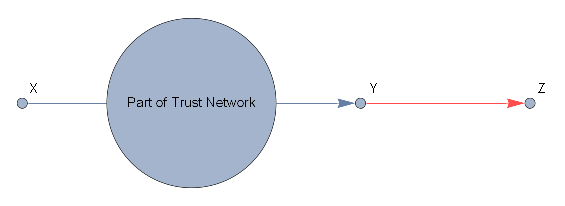
\includegraphics{export_gr1.eps}



More positive recommends never decrease the overall trust. More negative recommends never increase the overall trust.

\begin{equation}
x,y\in \mathcal{V},v\notin \mathcal{V}\overset{
\begin{array}{c}
 \mathcal{V}_*=\{x,y,v\} \\
 \mathcal{E}_*=\{(x,v),(v,y)\} \\
 \mathcal{G}_*=\left(\mathcal{V}_*,\mathcal{E}_*,A_*\right) \\
\end{array}
}{\to }f_{\mathcal{G}_*}(x,y)\left(f_{\mathcal{G}+\mathcal{G}_*}(x,y)-f_{\mathcal{G}}(x,y)\right)\geq 0
\end{equation}

(* DESCRIPTION NEEDED *)



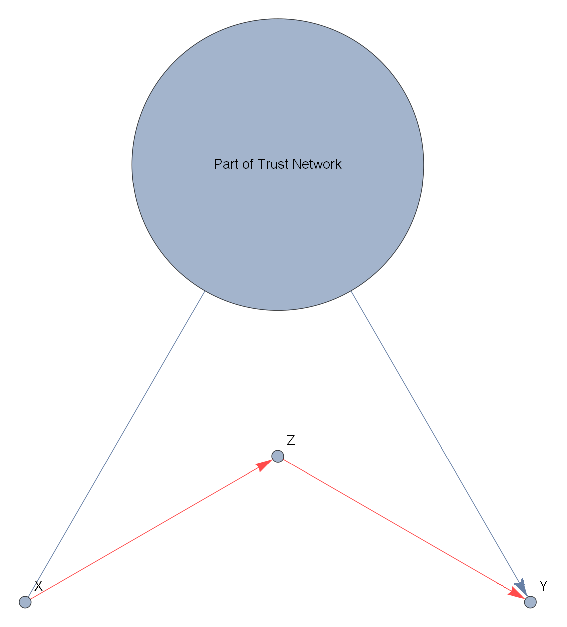
\includegraphics{export_gr2.eps}


\subsection{Trust Evaluation Function Discussion}

Here we discuss some solutions of trust evaluation function.

Normal Direct Reliable Trust

Let{'}s start at a very narrow scene, direct reliable trust. We only trust one with the exact direct trust value \(+1\) and ignore all the trust
value \(a\in [-1,0)\). Thus we have the following expression:

\begin{equation}
f_{\mathcal{G}}^{\text{NDRT}}(x,y)=\left\{
\begin{array}{cc}
 1 & a_{x,y}=1 \\
 0 & \text{else} \\
\end{array}
\right.
\end{equation}

Extended Direct Reliable Trust

Based on Normal Direct Reliable Trust, we can allow overall trust value \(-1\). Thus we have the following expression:

\begin{equation}
f_{\mathcal{G}}^{\text{EDRT}}(x,y)=\left\{
\begin{array}{cc}
 +1 & a_{x,y}=+1 \\
 -1 & a_{x,y}=-1 \\
 0 & \text{else} \\
\end{array}
\right.
\end{equation}

Normal Direct Reliable Threshold Trust

Based on Normal Direct Reliable Trust, we can use a threshold \(a_T\in (0,1)\) to decide whether an entity should be trusted. Thus we have the following
expression:

\begin{equation}
f_{\mathcal{G}}^{\text{NDRTT}}(x,y)=\left\{
\begin{array}{cc}
 1 & a_{x,y}\geq a_T \\
 0 & \text{else} \\
\end{array}
\right.
\end{equation}

Extended Direct Reliable Threshold Trust

Based on Extended Direct Reliable Trust, we can use a threshold \(a_T\in (0,1)\) to decide whether an entity should be trusted or distrusted. Thus
we have the following expression:

\begin{equation}
f_{\mathcal{G}}^{\text{EDRTT}}(x,y)=\left\{
\begin{array}{cc}
 +1 & a_{x,y}\geq a_T \\
 -1 & a_{x,y}\leq -a_T \\
 0 & \text{else} \\
\end{array}
\right.
\end{equation}

Extended Direct Unreliable Trust

We can use the direct trust value as the overall trust metric, in other words, trust has no transitivity. Thus we have the following expression:

\begin{equation}
f_{\mathcal{G}}^{\text{EDUT}}(x,y)=a_{x,y}
\end{equation}

Normal Direct Unreliable Trust

Based on Extended Direct Unreliable Trust, we can ignore the trust value \(a_T\in (0,1)\). Thus we have the following expression:

\begin{equation}
f_{\mathcal{G}}^{\text{NDUT}}(x,y)=\max \left(a_{x,y},0\right)
\end{equation}

Normal Recommended Reliable Trust

Based on Normal Direct Reliable Trust, we can assume trust can be passed from one entity to another. Thus we have the following expression:

\begin{equation}
f_{\mathcal{G},\mathit{p}}^{\text{NRRT}}(x,y)\overset{\left\{
\begin{array}{c}
 \mathit{p}_i=x \\
 \mathit{p}_j=y \\
\end{array}
\right.}{=}\left\{
\begin{array}{cc}
 \prod _{k=i}^{j-1} f_{\mathcal{G}}^{\text{NDRT}}\left(\mathit{p}_k,p_{k+1}\right) & i<j \\
 0 & \text{else} \\
\end{array}
\right.
\end{equation}

\begin{equation}
f_{\mathcal{G}}^{\text{NRRT}}(x,y)\overset{\mathcal{P}=\text{Permutations}(\mathcal{V})}{=}\left\{
\begin{array}{cc}
 1 & \exists \mathit{p}\in \mathcal{P},f_{\mathcal{G},\mathit{p}}^{\text{NRRT}}(x,y)=1 \\
 0 & \text{else} \\
\end{array}
\right.
\end{equation}

Extended Passive Recommended Reliable Trust

(* WHAT PASSIVE MEANS *)

Based on Normal Recommended Reliable Trust and Extended Direct Reliable Trust. We have the following expression:

\begin{equation}
f_{\mathcal{G},\mathit{p}}^{\text{ERRT}}(x,y)\overset{\left\{
\begin{array}{c}
 \mathit{p}_i=x \\
 \mathit{p}_j=y \\
\end{array}
\right.}{=}\left\{
\begin{array}{cc}
 \prod _{k=i}^{j-1} f_{\mathcal{G}}^{\text{EDRT}}\left(\mathit{p}_k,p_{k+1}\right) & i<j \\
 0 & \text{else} \\
\end{array}
\right.
\end{equation}

\begin{equation}
f_{\mathcal{G}}^{\text{EPRRT}}(x,y)\overset{\mathcal{P}=\text{Permutations}(\mathcal{V})}{=}\left\{
\begin{array}{cc}
 1 & \exists \mathit{p}\in \mathcal{P},f_{\mathcal{G},\mathit{p}}^{\text{ERRT}}(x,y)=1 \\
 0 & \text{else} \\
\end{array}
\right.
\end{equation}

Extended Initiative Recommended Reliable Trust

(* WHAT Initiative MEANS *)

Based on Extended Passive Recommended Reliable Trust and Extended Direct Reliable Trust. We have the following expression:

\begin{equation}
f_{\mathcal{G}}^{\text{EIRRT}}(x,y)\overset{\mathcal{P}=\text{Permutations}(\mathcal{V})}{=}\left\{
\begin{array}{cc}
 +1 & \left\{
\begin{array}{c}
 \exists \mathit{p}\in \mathcal{P},f_{\mathcal{G},\mathit{p}}^{\text{ERRT}}(x,y)=+1 \\
 \forall \mathit{p}\in \mathcal{P},f_{\mathcal{G},\mathit{p}}^{\text{ERRT}}(x,y)\neq -1 \\
\end{array}
\right. \\
 -1 & \left\{
\begin{array}{c}
 \exists \mathit{p}\in \mathcal{P},f_{\mathcal{G},\mathit{p}}^{\text{ERRT}}(x,y)=-1 \\
 \forall \mathit{p}\in \mathcal{P},f_{\mathcal{G},\mathit{p}}^{\text{ERRT}}(x,y)\neq +1 \\
\end{array}
\right. \\
 0 & \text{else} \\
\end{array}
\right.
\end{equation}

Recommended Unreliable Trust

Now let{'}s have a discussion about Recommended Unreliable Trust. First we have a strong assumption that trust evaluation can be built with two operations,
passing and combining. By comparing it to the matrix multiplication, we can define a multiplication operation of trust value adjacency matrix of
trust network \(\mathcal{G}\). \(\sum _*\) is the trust combining operation and \(\times _*\) is the trust combining operation. We will give some
definitions of \(\sum _*\) and \(\times _*\) later.

\begin{equation}
S\times T\overset{a_{i,j}=\underset{k\in \mathcal{V}}{\sum _*}s_{i,k}\times _*t_{k,j}}{=}\left(a_{i,j}\right)_{\mathcal{V}\times \mathcal{V}}
\end{equation}

Then we have the definition of the power of the trust value adjacency matrix of trust network \(\mathcal{G}\). Here \(n\) means the trust passing
steps.

\begin{equation}
A^n=A^{n-1}\times A
\end{equation}

We use \(\alpha _{i,j}\) to denote the entry in the \((i,j)\)-th position of \(A^n\). Thus we have the following expression to solve the overall
trust value from \(x\) to \(y\) with most \(n\) trust passing steps.

\begin{equation}
f_{\mathcal{G},n}^{\text{RUT}}(x,y)=\alpha _{x,y}
\end{equation}

Here we have a discussion about the properties of \(\sum _*\) and \(\times _*\).

\([-1,+1]\) are closed under both \(\sum _*\) and \(\times _*\).

\begin{equation}
\left\{a|a=\underset{k}{\sum _*}a_k,a_k\in [-1,+1]\right\}\subseteq [-1,+1]
\end{equation}

\begin{equation}
\left\{a|a=a_1\times _*a_2,a_1,a_2\in [-1,+1]\right\}\subseteq [-1,+1]
\end{equation}

Any increment of operand will never decrease the result on both \(\sum _*\) and \(\times _*\).

\begin{equation}
\frac{\partial \sum _*}{\partial a}\geq 0
\end{equation}

\begin{equation}
\frac{\partial \times _*}{\partial a}\geq 0
\end{equation}

We only discuss the \(\sum _*\) and \(\times _*\) operations on passive cases in the following. We can add some more assumptions.

Result of \(\sum _*\) is bigger than any operand and result of \(\times _*\) is smaller than any operand.

\[a_k\geq 0\to \underset{k}{\sum _*}a_k\geq \underset{k}{\max }\left(a_k\right)\]

\[a_1,a_2\geq 0\to a_1\times _*a_2\leq \min \left(a_1,a_2\right)\]

Here we give a simple example of \(\sum _*\) and \(\times _*\).

\[a_1,a_2\geq 0\to a_1\times _*a_2=a_1\times a_2\]

\[a_k\geq 0\to \underset{k}{\sum _*}a_k=e^{\frac{1}{\sum _k \frac{1}{\log \left(a_k\right)}}}\]

Here we give a simple solution of trust evaluation function about Recommended Unreliable Trust with most trust passing step 1.

\[\forall i,j\in \mathcal{V},a_{i,j}\geq 0\to f_{\mathcal{G},n}^{\text{RUT}}(x,y)=f_{\mathcal{G},1}^{\text{RUT}}(x,y)=e^{\frac{1}{\sum _{k\in \mathcal{V}}
\frac{1}{\log \left(a_{x,k}\times a_{k,y}\right)}}}\]

If we add some constraint on \(\sum _*\) and \(\times _*\) about associative property, commutative property and distributive property, we have the
following expression:

\[\underset{k=1,2}{\sum _*}a_k=\underset{k=2,1}{\sum _*}a_k\]

\[\underset{i}{\sum _*}\underset{j}{\sum _*}a_{i,j}=\underset{j}{\sum _*}\underset{i}{\sum _*}a_{i,j}\]

\[a_1\times _*a_2=a_2\times _*a_1\]

\[\left(a_1\times _*a_2\right)\times _*a_3=a_1\times _*\left(a_2\times _*a_3\right)\]

\[a\times _*\underset{k}{\sum _*}a_k=\underset{k}{\sum _*}a\times _*a_k\]

\[\left(\underset{k}{\sum _*}a_k\right)\times _*a=\underset{k}{\sum _*}\left(a_k\times _*a\right)\]

Here we give some simplest examples of { }\(\sum _*\) and \(\times _*\) satisfied the constraint above.

\[\left\{
\begin{array}{c}
 \sum _*=\max  \\
 \times _*=\min  \\
\end{array}
\right.\]

\[\left\{
\begin{array}{c}
 \sum _*=\max  \\
 \times _*=\times  \\
\end{array}
\right.\]

Although this result looks ridiculous, it is not useless. There may be lots of better solutions of trust evaluation functions and there should be
different trust evaluation functions under different scenarios. So we here only give some examples of trust evaluation functions. Trustor can customize
their own trust evaluation functions in their own way.


\section{Game Model}

We discussed the subjectiveness property and context-dependence property of our memoryless trust model. Then we will discuss the dynamism property.

The trust model is time-varying. We use \(\mathcal{G}^{(t)}\) to denote the trust network at time \(t\).

The backbone trust network is stored at the NEO main net as a state machine. We can use the operations on trust networks defined above to transform
it from \(\mathcal{G}^{(t)}\) to \(\mathcal{G}^{(t+1)}\) which means: anyone can join or leave the trust network; anyone can add or remove the trust
relation and update the trust value from himself to others.

There are three roles in the trust system: trustor, recommender, and trustee.

Here we discuss how the NEO-ID framework runs. When a trustor wants to verify the authenticity of the trustee, he has two options: passive mode and
initiative mode, of course he can also use both modes together.

Passive mode

the trustee make a request to the trustor; the trustor shows his trust profile to the trustee; the trustee gets trust proof from convenient recommenders;
the trustee submits the trust proof to the trustor; the trustor use his trust evaluation function to evaluate the overall trust to the trustee and
then make a decision.

Initiative mode

the trustee make a request to the trustor; the trust broadcasts the requests to some recommenders to verify the authenticity of the trustee; the
recommenders verify the authenticity of the trustee and submit the trust proof or broadcast the request to some other recommenders he trust or do
nothing; the trustor collects the trust proofs and make a decision.

Here we discuss the payoffs of the roles. (* DESCRIPTION NEEDED *)

\begin{equation}
\text{payoff}_{\text{TRUSTOR}}=\sum \left\{
\begin{array}{c}
 \text{payoff}_{\text{TRUSTOR},\text{TOPIC}} \\
 -\sum _{i\in \text{Recommenders}} \text{cost}_{\text{TRUSTOR},i} \\
 -\text{cost}_{\text{TRUSTOR},\text{SYSTEM}} \\
\end{array}
\right.
\end{equation}

\begin{equation}
\text{payoff}_{\text{RECOMMENDER}}=\sum \left\{
\begin{array}{c}
 \text{cost}_{\text{TRUSTOR},\text{RECOMMENDER}} \\
 \text{cost}_{\text{TRUSTEE},\text{RECOMMENDER}} \\
 -\text{cost}_{\text{RECOMMENDER},\text{SYSTEM}} \\
\end{array}
\right.
\end{equation}

\begin{equation}
\text{payoff}_{\text{TRUSTEE}}=\sum \left\{
\begin{array}{c}
 \text{payoff}_{\text{TRUSTEE},\text{TOPIC}} \\
 -\sum _{i\in \text{Recommenders}} \text{cost}_{\text{TRUSTEE},i} \\
 -\text{cost}_{\text{TRUSTEE},\text{SYSTEM}} \\
\end{array}
\right.
\end{equation}

In general, \(\text{cost}_{\text{TRUSTOR},\text{RECOMMENDER}}\) and \(\text{cost}_{\text{TRUSTEE},\text{RECOMMENDER}}\) will increase as the trust
value increases.

(* POSITIVE EXAMPLES $\&$ NEGITIVE EXAMPLES *)

(* REPUTATION is HERE *)

(* Additional management models *)


\section{Privacy Model}

(* What info is on blockchain *)

(* privacy level *)

(* Who can read the info *)

(* privacy and permission *)


\section{Protocol Design}

TRUST$\_$NETWORK represents a global trust network and it is stored on NEO blockchain. The data structure shows below.


\noindent \texttt{message TRUST$\_$NETWORK $\{$\\
\hspace*{2.ex} repeated ENTITY entities = 1;\\
\hspace*{2.ex} repeated AUTHORIZATION authorizations = 2;\\
\hspace*{2.ex} optional METADATA metadata = 3;\\
$\}$}

TRUST$\_$PROFILE stores the trust preferences of the trustor. It is not necessarily to be stored on blockchain, in other words, it is a local profile.


\noindent \texttt{message TRUST$\_$PROFILE $\{$\\
\hspace*{2.ex} repeated AUTHORIZATION authorizations = 1;\\
\hspace*{2.ex} optional TRUST$\_$EVALUATION$\_$FUNCTION trust$\_$evaluation$\_$function = 2;\\
\hspace*{2.ex} optional METADATA metadata = 3;\\
$\}$}

TRUST$\_$PROOF stores the recommendation information. It is not necessarily to be stored on blockchain, in other words, it is a local proof.


\noindent \texttt{message TRUST$\_$PROOF $\{$\\
\hspace*{2.ex} repeated AUTHORIZATION authorizations = 1;\\
\hspace*{2.ex} optional METADATA metadata = 3;\\
$\}$}

ENTITY represents an entity.


\noindent \texttt{message ENTITY $\{$\\
\hspace*{2.ex} ADDRESS address = 1;\\
\hspace*{2.ex} PUBLIC$\_$KEY public$\_$key = 2;\\
\hspace*{2.ex} ENTITY$\_$TYPE entity$\_$type = 3;\\
\hspace*{2.ex} repeated DOMAIN domains = 4;\\
\hspace*{2.ex} optional METADATA metadata = 5;\\
$\}$}

AUTHORIZATION represents an authorization.


\noindent \texttt{message AUTHORIZATION $\{$\\
\hspace*{2.ex} ADDRESS from = 1;\\
\hspace*{2.ex} ADDRESS to = 2;\\
\hspace*{2.ex} TRUST$\_$VALUE trust$\_$value = 3;\\
\hspace*{2.ex} VALID$\_$TIME valid$\_$time = 4;\\
\hspace*{2.ex} optional METADATA metadata = 5;\\
\hspace*{2.ex} SIGNATURE signature = 6;\\
$\}$}

ENTITY$\_$TYPE.


\noindent \texttt{message ENTITY$\_$TYPE $\{$\\
\hspace*{2.ex} TRUSTOR = 1;\\
\hspace*{2.ex} RECOMMENDER = 2;\\
\hspace*{2.ex} TRUSTEE = 3;\\
$\}$}


\section{Analysis}

(* TODO *)


\section{Conclusion}

(* TODO *)



\end{document}
